\documentclass[../differential_methods.tex]{subfiles}
\begin{document}
\section{Aula 01 - 22 de Fevereiro, 2026}
\subsection{Motivações}
\begin{itemize}
	\item Método das Diferenças Finitas;
	\item Método da Interpolação.
\end{itemize}
\subsection{Aproximações Numéricas das Derivadas}
O primeiro tópico a ser explorado são as aproximações finitas das derivadas de uma certa função u.
Vamos considerar, daqui adiante, uma função suficientemente suave, para que possamos diferenciar u(x) várias vezes, com cada uma delas sendo funções bem-definidas e limitadas em um intervalo, contendo algum ponto de interesse x.
Assim, por exemplo, para aproximar \(u'(\overline{x})\) por um método de aproximação por diferenças finitas, então podemos partir da definição de derivada
\[
	u'(\overline{x}) = \lim_{h\to 0} \frac{u(\overline{x}+h)-u(\overline{x})}{h},
\]
podemos tomar como referência esse quociente, considerar um h fixo e trocar a reta tangente no ponto pela reta secante, que corresponde a uma expressão do tipo
\[
	u'(\overline{x}) \approx D_{+}u(\overline{x})\coloneqq \frac{u(\overline{x}+h)-u(\overline{x})}{h};
\]
uma outra expressão com limite igualando a u' é
\[
	u'(\overline{x}) \approx D_{-}u(\overline{x})\coloneqq \frac{u(\overline{x})-u(\overline{x}-h)}{h},
\]
que corresponde à reta secante de pontos que vêm antes do \(\overline{x}\), com uma delas errando para mais e outra errando para menos, mas não são apenas essas -- também nos interessa, por exemplo, a média dessas duas aproximações! Afinal, se uma erra para mais e outra para menos, faz sentido considerar o meio termo, definindo o operador
\[
	u'(x)\approx D_{0}u(\overline{x})\coloneqq \frac{u(\overline{x}+h)-u(\overline{x}-h)}{h} = \frac{1}{2}[D_{+}u(\overline{x}) + D_{-}u(\overline{x})].
\]
Estes três operadores respectivamente levam os nomes de \textbf{operador de diferenças progressivo}, \textbf{operador de diferenças regressivo} e \textbf{operador de diferenças centrais}.
\begin{figure}[H]
	\begin{center}
		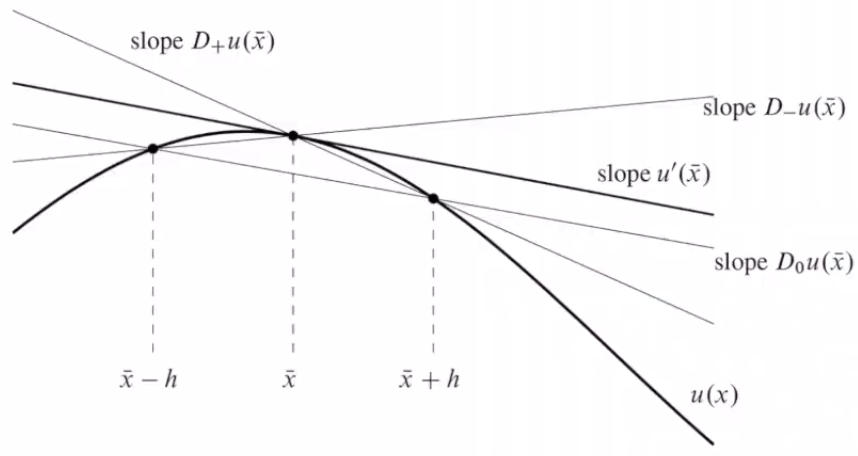
\includegraphics[height=0.7\textheight, width=0.7\textwidth, keepaspectratio]{./Images/slopes_01.png}
	\end{center}
	\caption{as inclinações vão se aproximando da tangente por baixo ou por cima de acordo com o operador escolhido!}
\end{figure}

Outras aproximações poderiam ser feitas, como uma considerando o terceiro termo de uma série expansiva, que veremos mais adiante, mas com expressão dada por
\[
	u'(\overline{x})\approx D_{3}u(\overline{x})\coloneqq \frac{1}{6h}[2u(\overline{x}+h)+3u(\overline{x})-6u(\overline{x}-h)-2u(\overline{x}-2h)],
\]
que envolve mais avaliações da função u.

Logo, um dos nosso objetivos será ver as diferenças, vantagens e desvantagens de cada uma dessas aproximações.

\begin{example}
	Considere uma função \(u(x)=\sin^{}{x}\) e o ponto \(\overline{x}=1\), cuja derivada no ponto 1 é o cosseno de 1, ou seja, queremos aproximar o ponto \(u'(1)=\cos^{}{(1)}=0.5403023\). A tabela abaixo mostra o erro e ordem dele de cada um dos operadores que vimos:
	\begin{table}[H]
		\centering
		\resizebox{\textwidth}{!}{
			\begin{tabular}{c | c c c c}
				\hline
				h       & \(D_{+}u(x)\) & \(D_{-}u(\overline{x})\) & \(D_{0} u(\overline{x})\) & \(D_{3}u(\overline{x})\) \\
				\hline
				1.0e-01 & -4.2939e-02   & 4.1138e-02               & -9.0005e-04               & 6.8207e-05               \\
				5.0e-02 & -2.1257e-02   & 2.0807e-02               & -2.2510e-04               & 8.6491e-06               \\
				1.0e-03 & -4.2163e-03   & 4.1983e-03               & -9.0050e-06               & 6.9941e-08               \\
				5.0e-03 & -2.1059e-03   & 2.1014e-03               & -2.2513e-06               & 8.7540e-09               \\
				1.0e-03 & -4.2083e-04   & 4.2065e-04               & -9.0050e-08               & 6.0979e-11               \\
				\hline
			\end{tabular}}
		\caption{erros em cada uma das diferentes aproximações finitas de \(u'(x).\)}
	\end{table}

	Por meio dela, percebemos que
	\begin{align*}
		 & D_{+}u(\overline{x})-u'(\overline{x})\approx -0.42h,          \\
		 & D_{0}u(\overline{x})-u'(\overline{x})\approx -0.09h^{2}, \;\& \\
		 & D_{3}u(\overline{x})-u'(\overline{x})\approx 0.007h^{3}.
	\end{align*}

	Com este exemplo, o que nos interessa é avaliar como essas formas de avaliar a derivada de formas diferentes se comportam conforme h fica menor, além de ver qual é o processo e a ordem de convergência de cada uma delas para o verdadeiro valor.
	O que vemos, primeiramente, é que as aproximações \(D_{+}\) e \(D_{-}\) são bem parecidas, mas com lineais opostos; a aproximação pela média, \(D_{0}\), produziu erros bem menores tanto comparada a \(D_{+}\) quanto a \(D_{-}\); mais ainda, a terceira aproximação, \(D_{3}\), ficou ainda mais precisa, com taxa de convergência mais rápida ainda!

\end{example}

Nós podemos fazer uma figura chamada \textbf{Teste de Convergência}, responsável por fornecer informações sobre as convergências das aproximações, que aparecerá para todos os tipos de aproximações que faremos; o \textbf{teste de convergência} em si é verificar qual é a taxa de convergência que estamos obtendo conforme h é refinada cada vez mais.
Assim, se o erro \(E(h)\) se comporta a uma taxa exponencial, por exemplo \(E(h)\approx C \cdot h^{p}\), então \(\log^{}{| E(h) |}\approx \log^{}{| C |} + p \log^{}{| h |},\) que traduz o gráfico outrora exponencial em um linear, facilitando as leituras que teremos; em relação às propriedades, para \(0<h_2<h_1\) aproximações suficientemente pequenas, esperamos que, por essa definição, \(E(h_1)\approx C h_1^{p}\) e \(E(h_2)\approx C h_{2}^{p}\), de modo que
\[
	\log^{}{\frac{| E(h_1) |}{| E(h_2) |}}\approx \log^{}{\frac{| C |h_{1}^{p}}{| C |h_{2}^{p}}} = \log^{}{\biggl(\frac{h_1}{h_2}\biggr)^{p}} = p \log^{}{\frac{h_1}{h_2}},
\]
ou seja, a ordem de convergência pode ser estimada por meio de
\[
	p\approx \frac{\log^{}{\biggl(\frac{| E(h_1) |}{| E(h_2) |}\biggr)}}{\log^{}{\biggl(\frac{h_1}{h_2}\biggr)}}.
\]

\begin{figure}[H]
	\begin{center}
		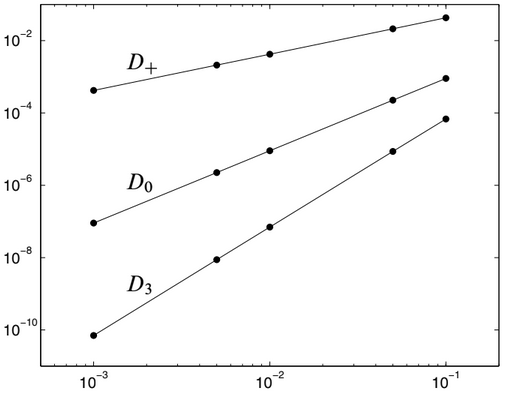
\includegraphics[height=0.7\textheight, width=0.7\textwidth, keepaspectratio]{./Images/convergence_test_01.png}
	\end{center}
	\caption{cada uma das linhas corresponde a um diferente valor da ordem de convergência p; aqui, a mais de cima seria o valor \(p=1\), seguido de \(p=2\) e \(p=3\).}
\end{figure}

Outro conceito importante de ser relembrado é a expansão de Taylor: se \(f\in \mathcal{C}^{n}([a, b])\) e existe a derivada \(f^{(n+1)}\) no intervalo \((a,b )\), então para quaisquer pontos c e x dentro do intervalo \([a, b]\), vale a expressão
\[
	f(x)=P_{n}(x)+E_{n}(x),
\]
onde \(P_{n}(x)\) é o \textbf{n-ésimo polinômio de Taylor}, dado por
\[
	P_{n}(x)\coloneqq \sum\limits_{k=0}^{n}\frac{1}{k!}f^{(k)}(c)(x-c)^{k}
\]
e o \textbf{termo residual/erro} \(E_{n}(x)\) é dado por
\[
	E_{n}(x)\coloneqq \frac{1}{(n+1)!}f^{(n+1)}(\zeta )(x-c)^{(n+1)},
\]
onde \(\zeta \) corresponde a algum ponto entre c e x.

Em vista das séries de Taylor, podemos também definir um conceito muito recorrente:
\begin{def*}
	Se \(f(h)\) e \(g(h)\) são duas funções em h, então diremos que \textbf{f é da ordem de g quando h tende a zero}, denotado por \(f(h)=\mathcal{O}(g(h))\) (``big-o de g'') se, para todo h suficientemente pequeno, vale
	\[
		| f(h) | \leq C | g(h) |. \; \square
	\]
\end{def*}
\begin{tcolorbox}[
		skin=enhanced,
		title=Observação,
		fonttitle=\bfseries,
		colframe=black,
		colbacktitle=cyan!75!white,
		colback=cyan!15,
		colbacklower=black,
		coltitle=black,
		drop fuzzy shadow,
		%drop large lifted shadow
	]
	O que a definição acima indica é que, se dividirmos f por g, esse valor vai ser constante a partir de certo h, correspondendo, então, a uma velocidade de decaimento para f:
	\[
		| f(h) |\leq C| g(h) | \Rightarrow \frac{| f(h) |}{| g(h) |}\leq C.
	\]
	Por exemplo, se \(f(h)=\mathcal{O}(h^{2})\), então f tende a zero tão rápido quanto uma função de ordem \(h^{2}\):
	\[
		| f(h) |\leq Ch^{2}.
	\]
	Para a maior parte das nossas aproximações, usaremos essa notação, dizendo que ela é da ordem de \(h^{p}\) para representar exatamente esta noção.
\end{tcolorbox}

Vamos ver, então, como ficam as ordens das aproximações ou \textbf{erros de truncação} das aproximações que vimos anteriormente.
\begin{example}[Operador \(D_{+}\)]
	Assuma que \(u\in \mathcal{C}^{2}([a, b])\), sendo x um ponto de \((a, b)\) e \(0<h<<1\); pelo Teorema de Taylor, vale a aproximaçÃo
	\[
		u(\overline{x}+h) = u(\overline{x})+hu'(\overline{x})+\frac{1}{2}h^{2}u''(\zeta ),
	\]
	para algum \( \zeta \in (\overline{x}, \overline{x}+h)\). Logo, temos
	\[
		u'(\overline{x})=\frac{u(\overline{x}+h)-u(\overline{x})}{h} - \frac{1}{2}hu''(\zeta ) = D_{+}u(\overline{x}) - \frac{1}{2}hu''(\zeta ).
	\]
	Consequentemente, ganhamos a relação
	\[
		| u'(\overline{x})-D_{+}u(\overline{x}) | =  \biggl\vert -\frac{1}{2}hu''(\zeta ) \biggr\vert\leq C| h | = Ch.
	\]
	Portanto, concluímos que o erro da aproximação pelo operador \(D_{+}(h)\) é da ordem h, ou seja, é um erro linear:
	\[
		u'(\overline{x})-D_{+}u(\overline{x})=\mathcal{O}(h) \Rightarrow u'(\overline{x})=D_{+}u(\overline{x})+\mathcal{O}(h).
	\]

	Esse exemplo ilustra as aproximações por diferenças finitas, porque passamos a representar o {\color{RoyalBlue3}operador derivada} de uma certa função por uma certa {\color{DeepPink2}fórmula de diferenças finitas} e um {\color{SpringGreen4} erro}:
	\[
		{\color{RoyalBlue3} \mathcal{D}u(\overline{x})} = {\color{DeepPink2}\mathcal{F}(\overline{x}, h)} + {\color{SpringGreen4}\mathcal{E}(\overline{x}, h)}.
	\]
	Neste caso específico, essa fórmula se traduz como
	\[
		{\color{RoyalBlue3} u'(\overline{x})} = {\color{DeepPink2}\frac{u(\overline{x}-h)-u(\overline{x})}{h}} + {\color{SpringGreen4}\mathcal{O}(h)}.
	\]
\end{example}
\begin{example}[Operador \(D_{-}\)]
	Agora, suponha que \(u\in \mathcal{C}^{2}([a, b])\), que x pertence a \((a, b)\) e que h é suficientemente pequeno, de modo que o Teorema de Taylor se aplica como
	\[
		u(\overline{x}-h) = u(\overline{x})-hu'(\overline{x})+\frac{1}{2}h^{2}u''(\zeta ), \quad \zeta \in (\overline{x}-h, \overline{x}).
	\]
	Portanto, pela mesma lógica, temos
	\begin{align*}
		u'(\overline{x})=\frac{u(\overline{x})-u(\overline{x}-h)}{h}+\frac{1}{2}hu''(\zeta ) & = D_{-}u(\overline{x})-\frac{1}{2}hu''(\zeta ) \\
		                                                                                     & = D_{-}u(\overline{x})+\mathcal{O}(h).
	\end{align*}
\end{example}

Pelos exemplos, ambas as aproximações indicam que o erro cai linearmente com h para as aproximações, mas esse nem sempre é o caso:
\begin{example}[Operador \(D_{0}\)]
	Vamos olhar a ordem do erro do operador \(D_{0}\). Aqui, nossas hipóteses são que u é uma função com pelo menos 3 derivadas (\(u\in \mathcal{C}^{3}([a, b])\)), enquanto que x e h são como antes.
	As expansões de Taylor deste exemplo são
	\begin{align*}
		 & u(\overline{x}+h)=u(\overline{x})+hu'(\overline{x})+\frac{1}{2}h^{2}u''(\overline{x})+\frac{1}{6}h^{3}u'''(\zeta_{1})  \\
		 & u(\overline{x}-h)=u(\overline{x})-hu'(\overline{x})+\frac{1}{2}h^{2}u''(\overline{x})-\frac{1}{6}h^{3}u'''(\zeta_{2}),
	\end{align*}
	onde \(\zeta_{1}\in (\overline{x}, \overline{x}+h)\) e \(\zeta_{2}\in (\overline{x}-h, \overline{x})\); logo, obtemos a expressão
	\begin{align*}
		u'(\overline{x}) & = \frac{u(\overline{x}+h)-u(\overline{x}-h)}{2h} - \frac{1}{2h}\frac{h^{3}}{6}(u'''(\zeta_1)+u'''(\zeta_{2})) \\
		                 & =D_{0}u(\overline{x})-\frac{h^{2}}{6}\frac{u'''(\zeta_{1})+u'''(\zeta_{2})}{2}.
	\end{align*}
	Neste caso, como o termo multiplicando \(\frac{h^{2}}{6}\) é médio entre \(u'''(\zeta_{1})\) e \(u'''(\zeta_{2})\), e como \(u\in \mathcal{C}^{3}([a, b])\), vale pelo \hyperlink{intermediate_value}{\textit{Teorema do Valor Intermediário}} que existe \(\zeta \) entre \(\zeta_{1}\) e \(\zeta_{2}\) (logo, \(\zeta \in (\overline{x}-h, \overline{x}+h)\)) tal que
	\[
		u'''(\zeta )=\frac{u'''(\zeta_{1})+u'''(\zeta_{2})}{2}.
	\]
	Portanto, a aproximação aqui obtida é do tipo
	\[
		u'(\overline{x})=D_{0}u(\overline{x})-\frac{h^{2}}{6}u'''(\zeta ) = D_{0}u(\overline{x}) + \mathcal{O}(h^{2}).
	\]
\end{example}

\begin{tcolorbox}[
		skin=enhanced,
		title=Lembrete!,
		after title={\hfill Teorema do Valor Intermediário},
		fonttitle=\bfseries,
		sharp corners=downhill,
		colframe=black,
		colbacktitle=yellow!75!white,
		colback=yellow!30,
		colbacklower=black,
		coltitle=black,
		%drop fuzzy shadow,
		drop large lifted shadow
	]
	O \hypertarget{intermediate_value}{Teorema do Valor Intermediário} pode ser enunciado como:\linebreak
	Seja \(f:[a, b]\rightarrow \mathbb{R}\) uma função contínua e tal que \(f(a)<f(b)\;(f(a)>f(b))\).\linebreak
	Se \(f(a)<k<f(b)\;(f(a)>k>f(b)),\)	então existe \(\overline{x}\in(a, b)\) tal que \(f(\overline{x})=k.\)
\end{tcolorbox}

\begin{example}[Operador \(D_{3}\)]
	Finalmente, repetindo o raciocínio para o operador \(D_{3}\), pedimos que \(u\in \mathcal{C}^{4}([a, b]),\; x\in (a, b)\) e \(0<h<<1\), precisaremos expandir os valores que entram na aproximação, ou seja, \(u(\overline{x}+h),\; u(\overline{x}-h)\) e \(u(\overline{x}-2h)\), resultando nas expansões de Taylor
	\begin{align*}
		 & u(\overline{x}+h)=u(\overline{x})+hu'(\overline{x})+\frac{1}{2}h^{2}u''(\overline{x})+\frac{1}{6}h^{3}u'''(\zeta_{1}) + \frac{1}{4!}h^{4}u^{(4)}(\zeta_{1})            \\
		 & u(\overline{x}-h)=u(\overline{x})-hu'(\overline{x})+\frac{1}{2}h^{2}u''(\overline{x})-\frac{1}{6}h^{3}u'''(\zeta_{2}) + \frac{1}{4!}h^{4}u^{(4)}(\zeta_{2})            \\
		 & u(\overline{x}-2h)=u(\overline{x})-2hu'(\overline{x})+\frac{1}{2}(2h)^{2}u''(\overline{x})-\frac{1}{6}(2h)^{3}u'''(\zeta_{2})+ \frac{1}{4!}(2h)^{4}u^{(4)}(\zeta_{3}),
	\end{align*}
	onde \(\zeta_{1}\in (\overline{x}, \overline{x}+h),\; \zeta_{2}\in (\overline{x}-h, \overline{x})\) e \(\zeta_{3}\in (\overline{x}-2h, \overline{x})\); logo, verifica-se que
	\begin{align*}
		u'(\overline{x}) & = \overbrace{\frac{1}{6h}\biggl[2u(\overline{x}+h) + 3u(\overline{x})-6u(\overline{x}-h)+u(\overline{x}-2h)\biggr]}^{D_{3}u(\overline{x})} \\
		                 & \quad - \frac{1}{6h}\biggl[\frac{2}{4!}h^{4}u^{(4)}(\zeta_{1})-\frac{6}{4!}h^{4}u^{(4)}+\frac{16}{4!}h^{4}u^{(4)}(\zeta_{3})\biggr]        \\
		                 & =D_{3}u(\overline{x})-\mathcal{O}(h^{3}).
	\end{align*}
\end{example}

Nós vimos como essas aproximações se comportam, susã importâncias e algumas delas; porém, dado um certo conjunto de pontos onde queremos aproximar a derivada, gostaríamos de determinar qual é a aproximação.
Para tanto, estudaremos, por meio do exemplo a seguir, o chamado \textbf{método dos coeficientes não determinados} -- suponha que queremos achar a aproximação por diferenças finitas de \(u'(\overline{x})\), digamos
\[
	u'(\overline{x})\approx D_{2}u(\overline{x}) \coloneqq au(\overline{x}) +bu(\overline{x}-h)+ cu(\overline{x}-2h),
\]
onde queremos determinar exatamente quem são os coeficientes a, b e c.

Utilizando a expansão de Taylor para \(u(\overline{x}-h)\) e \(u(\overline{x}-2h)\), chegamos à expressão
\[
	D_{2}u(\overline{x})=(a+b+c)u(\overline{x})-(b+2c)hu'(\overline{x})+\frac{1}{2}(b+4c)h^{2}u''(\overline{x})-\frac{1}{6}(b+8c)h^{3}u'''(\overline{x})+\mathcal{O}(h^{4});
\]
aqui, lembre-se da expressão das diferenças finitas -- precisamos que apareça, à direita do sinal de igual, o termo da derivada, e que os termos de ordem diferentes sumam, ou seja, queremos
\[
	\left\{\begin{array}{ll}
		a+b+c = 0, \text{ (zera o termo com função normal)}                 \\
		b+2c = -\frac{1}{h}, \text{ (isola o termo \(+u'(\overline{x})\))}, \\
		b+4c = 0, \text{ (zera o termo com derivada de ordem dois, garantindo mais precisão)}
	\end{array}\right.,
\]
enquanto que o termo com a derivada em ordem 3 representa o erro que desejamos, que faz ele permanecer não zerado.
Resolvendo esse sistema, obtemos:
\[
	a = \frac{3}{2h},\quad b = - \frac{2}{h},\quad\&\quad c = \frac{1}{2h},
\]
e chegamos à expressão
\[
	D_{2}u(\overline{x})=\frac{1}{2h}[3u(\overline{x})-4u(\overline{x}-h)+u(\overline{x}-2h)],
\]
tal que
\[
	{\color{DeepPink2}D_{2}u(\overline{x})}-{\color{RoyalBlue3}u'(\overline{x})} = {\color{SpringGreen4}-\frac{1}{6}(b+8c)h^{3}u'''(\overline{x})}+\mathcal{O}(h^{4})=-\frac{1}{3}h^{2}u'''(\overline{x})+\mathcal{O}(h^{3}) = \mathcal{O}(h^{2}).
\]

\begin{exr}
	Replique as ideias feitas acima para encontrar as aproximações com derivadas de ordens maiores!
\end{exr}

Existe um outro método que pode ser utilizado, conhecido como \textbf{Método da Interpolação}, onde consideramos que temos uma certa função \(u(x)\) e valores \(x_1 < x_2 < x_3\) com espaçamentos \(h_1 = x_2-x_1\) e \(h_2 = x_3-x_2\) de tamanhos diferentes; queremos obter a derivada de segunda ordem no ponto \(x_2\) usando uma combinação de valores \(u(x_1), u(x_2)\) e \(u(x_3)\).

Este método consiste em interpolar a função u e tomar as derivadas do polinômio aproximador ao invés dela. Um caso aqui é a forma de Newton para o polinômio interpolador, dada por
\[
	p(x)=U[x_1] + U[x_1, x_2] (x-x_1) + U[x_1, x_2, x_3](x-x_1)(x-x_2),
\]
onde \(U[\cdot ]\) representa as \textbf{diferenças divididas da função u}. Portanto, com este método,
\[
	u_{2}''(x_2)\approx p''(x_2) = 2 \underbrace{\frac{\frac{u(x_3)-u(x_2)}{h_2} - \frac{u(x_2)-u(x_1)}{h_1}}{h_1+h_2}}_{=U[x_1, x_2, x_3]} = c_1u(x_1)+c_2u(x_2)+c_3u(x_3),
\]
onde
\[
	c_1 = \frac{2}{h_1 (h_1+h_2)}, \quad c_2=-\frac{2}{h_1h_2} \quad\&\quad c_{3}=\frac{2}{h_2(h_1+h_2)}.
\]

\begin{exr}
	Compute o erro nessa aproximação expandindo \(u(x_1)\) e \(u(x_3)\) em séries de Taylor ao redor de \(x_2\). Além disso, pense no que acontece quando \(h_1=h_2\).
\end{exr}

Como último tópico dessa primeira aula, vamos ver como aproximar a derivada de ordem k de uma função \(u(\overline{x})\). A primeira coisa a se observar é que precisaremos de certa quantidade de pontos para fazer isso, especificamente um número suficiente para conseguirmos resolver as equações que irão surgir -- quando aproximamos a derivada de ordem 2, se usássemos apenas dois pontos, conseguiríamos eliminar o termo u e o u', mas não apareceria o ponto u'', ou seja, precisamos de no mínimo três pontos.
Em geral, precisamos de pelo menos \(n\geq k+1\) pontos, onde k é a ordem da derivada que desejamos aproximar; sendo assim, consideremos \(x_1,\dotsc ,x_{n}\) pontos distintos\footnote{O próprio \(\overline{x}\) pode ser um desses pontos, ou não.} e suponhamos que u seja suficientemente suave para que as séries de Taylor a seguir sejam válidas para cada \(i=1,\dotsc ,n:\)
\begin{align*}
	 & u(x_{1})=u(\overline{x})+(x_1-\overline{x})u'(\overline{x})+\dotsc + \frac{1}{k!}(x_1-\overline{x})^{k}u^{(k)}(\overline{x})+\dotsc  \\
	 & \quad \vdots                                                                                                                         \\
	 & u(x_{i})=u(\overline{x})+(x_i-\overline{x})u'(\overline{x})+\dotsc + \frac{1}{k!}(x_i-\overline{x})^{k}u^{(k)}(\overline{x})+\dotsc  \\
	 & \quad \vdots                                                                                                                         \\
	 & u(x_{n})=u(\overline{x})+(x_n-\overline{x})u'(\overline{x})+\dotsc + \frac{1}{k!}(x_n-\overline{x})^{k}u^{(k)}(\overline{x})+\dotsc.
\end{align*}
Lembremos que nosso objetivo é encontrar uma combinação linear destes valores que aproxime a derivada \(u^{(k)}(\overline{x})\), tal que
\[
	u^{(k)}(\overline{x})+\mathcal{O}(h^{p})=c_1u(x_1)+\dotsc +c_{n}u(x_{n}),
\]
com p quão grande quanto possível! Portanto,
\[
	\frac{1}{(i-1)!} \sum\limits_{j=1}^{n}c_{j}(x_{j}-\overline{x})^{(i-1)} = \left\{\begin{array}{ll}
		1, & \quad i-1=k       \\
		0, & \quad \text{c.c.}
	\end{array}\right.,
\]
onde \(i=1,\dotsc ,n\). Esta expressão define um sistema linear que precisamos resolver para encontrar os coeficientes \(c_1,c_2,\dotsc ,c_{n}\), e dado que \(x_1,x_2,\dotsc ,x_n\) são todos distintos, garantimos que o sistema de equações lineares é não singular e possui uma solução única!
\begin{tcolorbox}[
		skin=enhanced,
		title=Observação,
		fonttitle=\bfseries,
		colframe=black,
		colbacktitle=cyan!75!white,
		colback=cyan!15,
		colbacklower=black,
		coltitle=black,
		drop fuzzy shadow,
		%drop large lifted shadow
	]
	Se \(n\leq k\), com uma falta de pontos em nosso arcabouço, então o lado direito da equação e a solução ambos serão vetores nulos, mas para \(n>k\), os coeficientes fornecem uma aproximação de diferenças finitas adequada, como observado antes!

	A ordem p está relacionado exatamente com o número de pontos que temos (n) e a ordem d derivada que queremos aproximar (k), de modo que \(p\geq n-k\), mas não é uma igualdade: algumas situações de aproximações fazem com que o método tenha uma ordem maior que a esperada.
	Por exemplo, utilizando os pontos \(\overline{x},\; \overline{x}-h,\; \overline{x}-2h\), obtemos uma aproximação do tipo \(\mathcal{O}(h)\) para \(u'\); outra que fizemos foi \(\overline{x}-h, \; \overline{x}+h\) e \(\overline{x}\), da qual obtemos \(\mathcal{O}(h^{2})\).
	A diferença entre eles é que a segunda é simétrica, de forma que a expansão de Taylor dela cancela vários termos! Daí, a ordem acaba ficando maior que o esperado!
\end{tcolorbox}

\subsection{Calculando os Coeficientes}
Utilizando o MATLAB, podemos fazer um programa simples para retornar os coeficientes de uma aproximação por diferenças finitas utilizando a técnica generalizada que vimos. O código está abaixo, com comentários explicando as partes.

\begin{minted}[linenos=true, bgcolor=bg]{matlab}
 function c = findcoeff(k, xbar, x) % essa função leva como argumentos 
 %a ordem da derivada (k),  o ponto xbar onde ela será calculada,
 % e um vetor x com n posições contendo os pontos de x_1 até x_n,
 % e retorna o coeficiente c

 n = length(x); % obtém o tamanho do vetor x

 A = ones(n, n); % inicializa uma matriz n por n de 1s,   
 % pois não queremos que tenha entradas 0, todas serão preenchidas 

 xrow = (x-xbar); % um vetor resultando das diferenças entre 
 % as entradas x_j  do vetor x e o escalar xbar. 
 % Cuidado com a orientação do vetor x: aqui, supomos que sempre  
 % entramos com um vetor linha.

 % Precisamos percorrer a matriz A 
 % e determinar os valores que ela recebe em cada linha:
 for i=2:n % como o resultado da operação abaixo para a linha 
 % 1 vai ser um monte de 1, podemos começar a partir da 2
    A(i, :) = (xrow .^ (i-1)) ./ factorial(i-1); 
    % buscamos evitar um loop interno j, 
    % então faremos uma operação vetorial: 
    % na linha i, definiremos todas as colunas da matriz A, 
    % como indicado pelo ``:'' na segunda entrada. 
    % A expressão ``.^'' indica que a exponenciação fará com que
    % cada entrada seja elevada a i-1,
    % e a ``./'' faz com que todos os
    % termos sejam divididos pelo fatorial de i-1.
 end 

 % Agora, vamos definir o lado direito.

 b = zeros(n, 1); % vetor de n linhas e 1 coluna com zeros.
 b(k+1) = 1; % quando i for k+1, ou seja, em b(k+1), inserimos 1.

 c = A \ b; % retorna c tal que (Ac)=b, 
 % e a barra invertida é o comando do MATLAB para resolver um 
 % sistema linear. Muito mais otimizado do que fazer inv(A)*b.

 c = c'; % transpões c para evitar problemas de compatibilidade.
 
 end
 \end{minted}
Ao fazer os programas, evite fazer como fiz acima! Os comentários são puramente didáticos, isso deixa o código muito poluído como deu pra ver.
Teste o programa depois de fazer ele! Por exemplo, rode \textit{fdcoeff(1, 1, x)}, com \textit{x(1)=1 e x(2)=1+h, h=0.05}, ou então \textit{c = fdcoeff(1,1, sin(x))} e fazer \(ad = c * u'\).

\end{document}
